\section{Rule-Based Classification}

\begin{frame}{Basic Concepts}
	\begin{itemize}
		\item Rule-based classification is based on a set of \textbf{IF-THEN rules}.
		\item Each \textbf{IF-THEN rule} consists of two parts:
		      \begin{itemize}
			      \item \textbf{\color{airforceblue}IF} (antecedent/precondition): a condition or set of conditions that must be satisfied.
			      \item \textbf{\color{airforceblue}THEN} (consequent): the conclusion or action that follows if the IF part is satisfied.
		      \end{itemize}
		      \visible<2->{
		\item \textbf{Example:} (one rule)
		      \begin{itemize}
			      \item \textbf{IF} \texttt{age} $\leq$ 30 AND \texttt{student} = "yes" \textbf{THEN} \texttt{buys\_computer} = "yes".
		      \end{itemize}
		      }
		      \visible<3->{
		\item Very \textbf{easy} to read and understand for humans.
		      }
	\end{itemize}
\end{frame}

\begin{frame}{Example}
	\begin{itemize}
		\item Given is a \textbf{\color{airforceblue}set of rules}:
		      \begin{itemize}
			      \item \textbf{IF} \texttt{price} $<$ 1500 \textbf{THEN} \texttt{buy} = "yes".
			      \item \textbf{IF} \texttt{price} $\geq$ 1500 AND \texttt{color} = "red" \textbf{THEN} \texttt{buy} = "no".
			      \item \textbf{IF} \texttt{price} $\geq$ 1500 AND \texttt{location} = "Erlangen" \textbf{THEN} \texttt{buy} = "yes".
		      \end{itemize} \medskip
		      \visible<2->{
		\item The set may be used to classify \textbf{\color{airforceblue}new tuples}: \medskip
		      \begin{center}
			      \scalebox{0.85}{
				      \begin{tabular}{|c|c|c|c|}
					      \hline
					      \rowcolor{faugray!62}\textbf{price}                                 & \textbf{color}                                                       & \textbf{location}                                                       & \textbf{buy}                                                                   \\\hline
					      % Scenario 1: Exactly one rule is triggered
					      \only<3-4>{\cellcolor{faugray!28}}1349                              & \only<3-4>{\cellcolor{faugray!28}}red                                & \only<3-4>{\cellcolor{faugray!28}}Nuremberg                             & \only<3-4>{\cellcolor{faugray!28}}\only<-3>{?}\only<4->{{\color{faugreen}yes}} \\\hline
					      % Scenario 2: More than one rule is triggered
					      \only<5>{\cellcolor{faugray!28}}\only<6>{\cellcolor{faured!28}}2306 & \only<5>{\cellcolor{faugray!28}}\only<6>{\cellcolor{faured!28}}red   & \only<5>{\cellcolor{faugray!28}}\only<6>{\cellcolor{faured!28}}Erlangen & \only<5>{\cellcolor{faugray!28}}\only<6>{\cellcolor{faured!28}}?
					      \\\hline
					      % Scenario 3: No rule is triggered
					      \only<7>{\cellcolor{faugray!28}}\only<8>{\cellcolor{faured!28}}1995 & \only<7>{\cellcolor{faugray!28}}\only<8>{\cellcolor{faured!28}}green & \only<7>{\cellcolor{faugray!28}}\only<8>{\cellcolor{faured!28}}Fuerth   & \only<7>{\cellcolor{faugray!28}}\only<8>{\cellcolor{faured!28}}?
					      \\\hline
				      \end{tabular}
			      }
		      \end{center}
		      } \medskip

		      \visible<6->{
		\item Some scenarios might lead to \textbf{\color{airforceblue}conflicts}:
		      \begin{enumerate}
			      \item More than one rule is triggered.
			            \visible<8->{
			      \item No rule is triggered.
			            }
		      \end{enumerate}
		      }

	\end{itemize}

\end{frame}

\begin{frame}{Potential Solutions}
	\begin{enumerate}
		\item \textbf{More than one rule is triggered: {\color{airforceblue}conflict resolution}.}
		      \begin{itemize}
			      \item \textbf{\color{airforceblue}Size ordering:}
			            \begin{itemize}
				            \item Assign the highest priority to the triggered rule that has the "toughest" requirement \\ (i.e., rule with most used attribute in condition).
			            \end{itemize}
			      \item \textbf{\color{airforceblue}Class-based ordering:}
			            \begin{itemize}
				            \item Decreasing order of prevalence or misclassification cost per class.
				            \item No order of rules within class $\rightarrow$ disjunction (logical \texttt{OR}) between rules.
			            \end{itemize}
			      \item \textbf{\color{airforceblue}Rule-based ordering} (decision list):
			            \begin{itemize}
				            \item Rules are organized into one long priority list,\\
				                  according to some measure of rule quality, or by experts.
				            \item Rules \underline{must} be applied in this particular order to avoid conflict.
			            \end{itemize}
		      \end{itemize}
		      \visible<2->{
		\item \textbf{No rule is triggered.}
		      \begin{itemize}
			      \item Use a fallback/default rule.
			      \item Always evaluated as the last rule, if and only if other rules are not covered by some tuple, i. e. no rules have been triggered.
		      \end{itemize}
		      }
	\end{enumerate}
\end{frame}

\begin{frame}{Rule Extraction from a Decision Tree}
	\begin{itemize}
		\item \textbf{Basic idea:}
		      \begin{itemize}
			      \item Rules are \textbf{\color{airforceblue}easier to understand} than large trees.
			      \item A rule can be created for \textbf{\color{airforceblue}each path from the root to a leaf.}
			      \item Each attribute-value pair along the path forms \textbf{\color{airforceblue}a condition}:
		      \end{itemize}
	\end{itemize}
	\vspace*{0em}
	\visible<2->{
		\begin{center}
			\begin{columns}
				\begin{column}{0.45\textwidth}
					\begin{figure}[h]
						\centering
						\scalebox{0.9}{
							\begin{tikzpicture}[
		overlay,
		remember picture,
		>=latex,
		thick,
		node/.style={
				draw=faugray,
				rounded corners=.25em,
				fill=faugray!62,
				text depth=0.2em
			},
		leaf/.style={
				draw,
				rounded corners=.7em,
				text depth=0.2em
			},
		branch/.style={
				fill=white,
				font=\ttfamily\scriptsize,
				rounded corners=.7em,
				text depth=0.2em
			}
	]
	\node[node] at (0,0) (age) {age?};
	\node[leaf,text=faugreen,below=6.2em of age] (age-yes) {yes};

	\node[node,below left=2em and 1.5em of age] (student) {student?};
	\node[leaf,text=faured,below right=2.5em and -1em of student] (student-no) {no};
	\node[leaf,text=faugreen,below left=2.5em and -1em of student] (student-yes) {yes};

	\node[node,below right=2em and .6em of age] (credit-rating) {credit rating?};
	\node[leaf,text=faured,below left=2.5em and -2em of credit-rating] (credit-no) {no};
	\node[leaf,text=faugreen,below right=2.5em and -2em of credit-rating] (credit-yes) {yes};

	\draw (age.south) -- (age-yes.north);
	\node[branch,below=4em of age.north] {31\dots 40};

	\draw[rounded corners=5pt]
	(age.south) -- ($(age.south) + (0,-1em)$) --
	($(student.north) + (0,1em)$) -- (student.north);
	\node[branch,above=1em of student.north] {$\leq$30};

	\path[draw,rounded corners=5pt]
	(age.south) -- ($(age.south) + (0,-1em)$) --
	($(credit-rating.north) + (0,1em)$) -- (credit-rating.north);
	\node[branch,above=1em of credit-rating.north] {>40};

	% student labels
	\draw[rounded corners=5pt]
	(student.south) -- ($(student.south) + (0,-1.5em)$) --
	($(student-no.north) + (0,1em)$) -- (student-no.north);
	\node[branch,above=1em of student-no.north] {no};

	\draw[rounded corners=5pt]
	(student.south) -- ($(student.south) + (0,-1.5em)$) --
	($(student-yes.north) + (0,1em)$) -- (student-yes.north);
	\node[branch,above=1em of student-yes.north] {yes};

	% credit-rating labels
	\draw[rounded corners=5pt]
	(credit-rating.south) -- ($(credit-rating.south) + (0,-1.5em)$) --
	($(credit-no.north) + (0,1em)$) -- (credit-no.north);
	\node[branch,above=1em of credit-no.north] {excellent};

	\draw[rounded corners=5pt]
	(credit-rating.south) -- ($(credit-rating.south) + (0,-1.5em)$) --
	($(credit-yes.north) + (0,1em)$) -- (credit-yes.north);
	\node[branch,above=1em of credit-yes.north] {fair};
\end{tikzpicture}

						}
					\end{figure}
				\end{column}
				\begin{column}{0.45\textwidth}
					\begin{enumerate}
						\visible<3->{
						\item \textbf{IF} \texttt{age} $\leq$ 30 AND \texttt{student} = "yes" \\
						      \textbf{THEN} \texttt{buys\_computer} = "yes".
						      }
						      \visible<4->{
						\item \textbf{IF} \texttt{age} $\leq$ 30 AND \texttt{student} = "no" \\
						      \textbf{THEN} \texttt{buys\_computer} = "no".
						      }
						      \visible<5->{
						\item \textbf{IF} \texttt{age}= $31\ldots40$ \\
						      \textbf{THEN} \texttt{buys\_computer} = "yes".
						      }
						      \visible<6->{
						\item \dots
						      }
					\end{enumerate}
				\end{column}
			\end{columns}
		\end{center}
	}
\end{frame}

\begin{frame}{Rule Induction: Sequential Covering Method}
	\begin{itemize}
		\item Extracting rules from decision trees is not \textbf{the only} way to learn rules.
		\item Rules can be learned \textbf{\color{airforceblue}directly} from \textbf{\color{airforceblue}the training data}:
		      \begin{itemize}
			      \item Rules are learned \textbf{sequentially}.
			      \item Each rule is optimized to cover \textbf{as many tuples of a given class} as possible\\ while covering \textbf{as few tuples of other classes} as possible.
		      \end{itemize}
	\end{itemize}

	\visible<2->{
		\begin{center}
			\begin{columns}
				\begin{column}{0.45\textwidth}
					\begin{itemize}
						\item \textbf{Steps of the method:}
						      \begin{enumerate}
							      \visible<3->{
							      \item Start with an empty set of rules.
							            }
							            \visible<4->{
							      \item Find the rule $r$ with the best covering.
							            }
							            \visible<5->{
							      \item Removed all tuples covered.
							            }
							            \visible<6->{
							      \item Repeat with step 2 until:
							            \begin{itemize}
								            \item No more tuples left.
								            \item The quality of a rule is below a threshold.
							            \end{itemize}
							            }
						      \end{enumerate}
					\end{itemize}

				\end{column}
				\begin{column}{0.45\textwidth}
					\begin{center}
						\newcommand*{\xMin}{0}%
						\newcommand*{\xMax}{8}%
						\newcommand*{\yMin}{0}%
						\newcommand*{\yMax}{5}%
						\newcommand*{\colorOne}{faured}%
						\newcommand*{\colorTwo}{faugray}%
						\begin{tikzpicture}[scale=0.5]
							\foreach \i in {\xMin,...,\xMax} {
									\draw [very thin,gray] (\i,\yMin) -- (\i,\yMax)  node [below] at
									(\i,\yMin) {\tiny$\i$};
								}
							\foreach \i in {\yMin,...,\yMax} {
									\draw [very thin,gray] (\xMin,\i) -- (\xMax,\i) node [left] at
									(\xMin,\i) {\tiny$\i$};
								}
							% \colorOne Nodes (35)
							\node[circle,fill=\colorOne,scale=0.5] at (0.7,0.8) {};
							\node[circle,fill=\colorOne,scale=0.5] at (1.2,1.3) {};
							\node[circle,fill=\colorOne,scale=0.5] at (0.9,2.1) {};
							\node[circle,fill=\colorOne,scale=0.5] at (1.5,3.2) {};
							\node[circle,fill=\colorOne,scale=0.5] at (1.8,1.7) {};
							\node[circle,fill=\colorOne,scale=0.5] at (2.1,0.9) {};
							\node[circle,fill=\colorOne,scale=0.5] at (2.3,1.4) {};
							\node[circle,fill=\colorOne,scale=0.5] at (1.9,2.3) {};
							\node[circle,fill=\colorOne,scale=0.5] at (0.8,3.5) {};
							\node[circle,fill=\colorOne,scale=0.5] at (1.3,4.2) {};
							\node[circle,fill=\colorOne,scale=0.5] at (2.2,4.1) {};
							\node[circle,fill=\colorOne,scale=0.5] at (2.4,3.3) {};
							\node[circle,fill=\colorOne,scale=0.5] at (3.2,1.1) {};
							\node[circle,fill=\colorOne,scale=0.5] at (3.7,0.7) {};
							\node[circle,fill=\colorOne,scale=0.5] at (4.1,1.5) {};
							\node[circle,fill=\colorOne,scale=0.5] at (4.6,0.9) {};
							\node[circle,fill=\colorOne,scale=0.5] at (5.3,1.2) {};
							\node[circle,fill=\colorOne,scale=0.5] at (5.9,0.8) {};
							\node[circle,fill=\colorOne,scale=0.5] at (6.2,1.4) {};
							\node[circle,fill=\colorOne,scale=0.5] at (6.7,0.9) {};
							\node[circle,fill=\colorOne,scale=0.5] at (7.1,1.6) {};
							\node[circle,fill=\colorOne,scale=0.5] at (6.8,2.3) {};
							\node[circle,fill=\colorOne,scale=0.5] at (7.2,3.1) {};
							\node[circle,fill=\colorOne,scale=0.5] at (6.5,3.7) {};
							\node[circle,fill=\colorOne,scale=0.5] at (7.3,4.2) {};
							\node[circle,fill=\colorOne,scale=0.5] at (5.8,4.3) {};
							\visible<-4>{\node[circle,fill=\colorOne,scale=0.5] at (5.1,3.9) {};}
							\node[circle,fill=\colorOne,scale=0.5] at (3.1,2.3) {};
							\node[circle,fill=\colorOne,scale=0.5] at (4.4,2.4) {};
							\node[circle,fill=\colorOne,scale=0.5] at (3.8,2.1) {};
							\node[circle,fill=\colorOne,scale=0.5] at (4.2,1.8) {};
							\node[circle,fill=\colorOne,scale=0.5] at (4.9,2.2) {};
							\visible<-4>{\node[circle,fill=\colorOne,scale=0.5] at (2.4,2.7) {};}
							\visible<-4>{\node[circle,fill=\colorOne,scale=0.5] at (3.9,3.2) {};}
							\visible<-4>{\node[circle,fill=\colorOne,scale=0.5] at (5.4,2.9) {};}

							% \colorTwo Nodes (45)
							\node[circle,fill=\colorTwo,scale=0.5] at (1.1,1.9) {};
							\node[circle,fill=\colorTwo,scale=0.5] at (1.7,2.7) {};
							\node[circle,fill=\colorTwo,scale=0.5] at (2.9,2.2) {};
							\visible<-4>{\node[circle,fill=\colorTwo,scale=0.5] at (2.9,2.7) {};}
							\visible<-4>{\node[circle,fill=\colorTwo,scale=0.5] at (3.1,2.9) {};}
							\visible<-4>{\node[circle,fill=\colorTwo,scale=0.5] at (3.4,3.2) {};}
							\visible<-4>{\node[circle,fill=\colorTwo,scale=0.5] at (3.7,3.6) {};}
							\visible<-4>{\node[circle,fill=\colorTwo,scale=0.5] at (3.9,4.1) {};}
							\visible<-4>{\node[circle,fill=\colorTwo,scale=0.5] at (3.3,3.8) {};}
							\visible<-4>{\node[circle,fill=\colorTwo,scale=0.5] at (2.8,3.5) {};}
							\visible<-4>{\node[circle,fill=\colorTwo,scale=0.5] at (2.7,4.0) {};}
							\visible<-4>{\node[circle,fill=\colorTwo,scale=0.5] at (3.2,4.3) {};}
							\visible<-4>{\node[circle,fill=\colorTwo,scale=0.5] at (3.8,2.8) {};}
							\visible<-4>{\node[circle,fill=\colorTwo,scale=0.5] at (4.1,3.1) {};}
							\visible<-4>{\node[circle,fill=\colorTwo,scale=0.5] at (4.3,3.5) {};}
							\visible<-4>{\node[circle,fill=\colorTwo,scale=0.5] at (4.6,3.9) {};}
							\visible<-4>{\node[circle,fill=\colorTwo,scale=0.5] at (4.8,4.2) {};}
							\visible<-4>{\node[circle,fill=\colorTwo,scale=0.5] at (4.5,2.8) {};}
							\visible<-4>{\node[circle,fill=\colorTwo,scale=0.5] at (4.9,3.3) {};}
							\visible<-4>{\node[circle,fill=\colorTwo,scale=0.5] at (5.2,3.6) {};}
							\visible<-4>{\node[circle,fill=\colorTwo,scale=0.5] at (5.4,4.1) {};}
							\visible<-4>{\node[circle,fill=\colorTwo,scale=0.5] at (5.1,2.7) {};}
							\node[circle,fill=\colorTwo,scale=0.5] at (2.6,1.2) {};
							\node[circle,fill=\colorTwo,scale=0.5] at (2.9,1.8) {};
							\node[circle,fill=\colorTwo,scale=0.5] at (3.4,1.9) {};
							\node[circle,fill=\colorTwo,scale=0.5] at (4.3,2.1) {};
							\node[circle,fill=\colorTwo,scale=0.5] at (4.8,1.8) {};
							\node[circle,fill=\colorTwo,scale=0.5] at (5.7,1.9) {};
							\node[circle,fill=\colorTwo,scale=0.5] at (6.1,2.1) {};
							\node[circle,fill=\colorTwo,scale=0.5] at (6.3,2.8) {};
							\node[circle,fill=\colorTwo,scale=0.5] at (6.4,3.3) {};
							\node[circle,fill=\colorTwo,scale=0.5] at (5.7,3.4) {};
							\node[circle,fill=\colorTwo,scale=0.5] at (0.7,1.4) {};
							\node[circle,fill=\colorTwo,scale=0.5] at (0.9,3.1) {};
							\node[circle,fill=\colorTwo,scale=0.5] at (1.4,3.8) {};
							\node[circle,fill=\colorTwo,scale=0.5] at (7.0,1.0) {};
							\node[circle,fill=\colorTwo,scale=0.5] at (6.9,3.4) {};
							\visible<-4>{\node[circle,fill=\colorTwo,scale=0.5] at (4.2,2.6) {};}
							\visible<-4>{\node[circle,fill=\colorTwo,scale=0.5] at (3.6,2.6) {};}
							\visible<-4>{\node[circle,fill=\colorTwo,scale=0.5] at (4.7,3.6) {};}
							\visible<-4>{\node[circle,fill=\colorTwo,scale=0.5] at (3.5,4.0) {};}
							\visible<-4>{\node[circle,fill=\colorTwo,scale=0.5] at (4.1,3.7) {};}
							\visible<-4>{\node[circle,fill=\colorTwo,scale=0.5] at (4.4,4.1) {};}
							\visible<-4>{\node[circle,fill=\colorTwo,scale=0.5] at (5.0,3.1) {};}
							\visible<-4>{\node[circle,fill=\colorTwo,scale=0.5] at (3.8,3.3) {};}
							\visible<-4>{\node[circle,fill=\colorTwo,scale=0.5] at (2.8,3.1) {};}

							\node[very thin,black,right] at (\xMax + 0.5, \yMax - 0.5) (l) {\scriptsize Legend:};

							\node[circle,fill=\colorOne,scale=0.5,below=1mm of l] (ptw) {};
							\node[very thin,black,right=0.25mm of ptw] {\scriptsize Class 1};
							\node[circle,fill=\colorTwo,scale=0.5,below=1mm of ptw] (pth) {};
							\node[very thin,black,right=0.25mm of pth] {\scriptsize Class 2};


							\visible<4->{
								% Major Class 2 Area
								\draw[thick, dashed, faugraydark] (2.5, 2.5) rectangle (5.5, 4.5);
							}

							\visible<6->{
								% Major Class 1 Area
								\draw[thick, dashed, faureddark] (3, 0.5) rectangle (6.8, 1.7);
							}
						\end{tikzpicture}
					\end{center}
				\end{column}
			\end{columns}
		\end{center}
	}
\end{frame}

\begin{frame}{Rule Induction: Sequential Covering Method}
	\begin{itemize}
		\item \textbf{Sequential covering algorithm:}
		      \begin{itemize}
			      \item Extracts rules directly from training data.
		      \end{itemize}
		\item \textbf{Typical sequential covering algorithms:}
		      \begin{itemize}
			      \item FOIL, AQ, CN2, RIPPER.
		      \end{itemize}
		\item \textbf{Rules are learned {\color{airforceblue}sequentially}.}
		      \begin{itemize}
			      \item Each rule for a given class $C_i$ will cover many tuples of $C_i$, but none (or few) of the tuples of other classes.
		      \end{itemize}
		\item \textbf{Algorithm sketch:}
		      \begin{itemize}
			      \item Rules are learned one at a time.
			      \item Each time a rule is learned, the tuples covered by the rule are removed.
			      \item The process repeats on the remaining tuples unless termination condition, e.g., when no more training examples left or when the quality of a rule returned is below a user-specified threshold.
		      \end{itemize}
		\item \textbf{Compare with decision-tree induction:}
		      \begin{itemize}
			      \item That was learning a set of rules simultaneously.
		      \end{itemize}
	\end{itemize}
\end{frame}

\begin{frame}{Sequential Covering Algorithm (I)}
	\begin{algorithm}[H]
		\SetAlgoVlined
		\KwData{
			\begin{itemize}
				\item Training dataset $D$ containing tuples with their associated class labels;
				\item \texttt{attribute\_values}, the set of all attributes and their possible values;
			\end{itemize}
		}
		\KwResult{A rule set.}
		\BlankLine
		\texttt{rule\_set} $\leftarrow \{\}$ \tcp*[l]{Initial set of rules learned is empty}
		\BlankLine
		\ForEach{class $c$ of $D$}{
			\Repeat{terminating condition}{
				\texttt{rule} $\leftarrow$ \texttt{learn\_one\_rule}($D$, \texttt{attribute\_values, $c$})\;
				remove tuples covered by \texttt{rule} from $D$\;
				\BlankLine
				\texttt{rule\_set} $\leftarrow$ \texttt{rule\_set} + \texttt{rule} \tcp*[l]{add new rule to rule set}
			}
		}
		\BlankLine
		\KwRet{
			\texttt{rule\_set}\;
		}
	\end{algorithm}
\end{frame}

\begin{frame}{Sequential Covering Algorithm (II)}
	\begin{itemize}
		\item Rules are learned in a \textit{general-to-specific} manner
		\item Start with the most general rule possible: a rule with an empty condition
		      \begin{center}
			      IF THEN \texttt{buys\_computer} = "yes"
		      \end{center}
		\item Then: Consider each possible attribute (\texttt{attribute\_values})\newline
		      For instance: attribute-value pair (\texttt{att}, \texttt{val}); consider the following attribute tests:\newline
		      \texttt{att} = \texttt{val}, \texttt{att} $<$ \texttt{val}, \texttt{att} $\leq$ \texttt{val}, \texttt{att} > \texttt{val}, \texttt{att} $\geq$ \texttt{val}
		\item \textbf{Curse of dimensionality:} testing each attribute-value pair is computationally explosive
		\item Solution: \textbf{greedy depth-first strategy of \texttt{learn\_one\_rule}}
		      \begin{itemize}
			      \item Add new attribute test that improves the rule quality the most.
			      \item Each time a new attribute test is added, the rule should cover more "accept" tuples (\texttt{buys\_computer} = "yes").
			      \item Repeat until a certain acceptable quality level is reached (\textit{terminating condition}).
		      \end{itemize}
		\item \textbf{What if we added a poor choice?} Greedy search does not allow for backtracking.
		      \begin{itemize}
			      \item Retain the best $k$ attribute candidates at each step, rather than a single best candidate.
		      \end{itemize}
	\end{itemize}
\end{frame}

\begin{frame}{Sequential Covering Algorithm (III)}
	\vspace*{-1em}
	\begin{figure}[h]
		\centering
		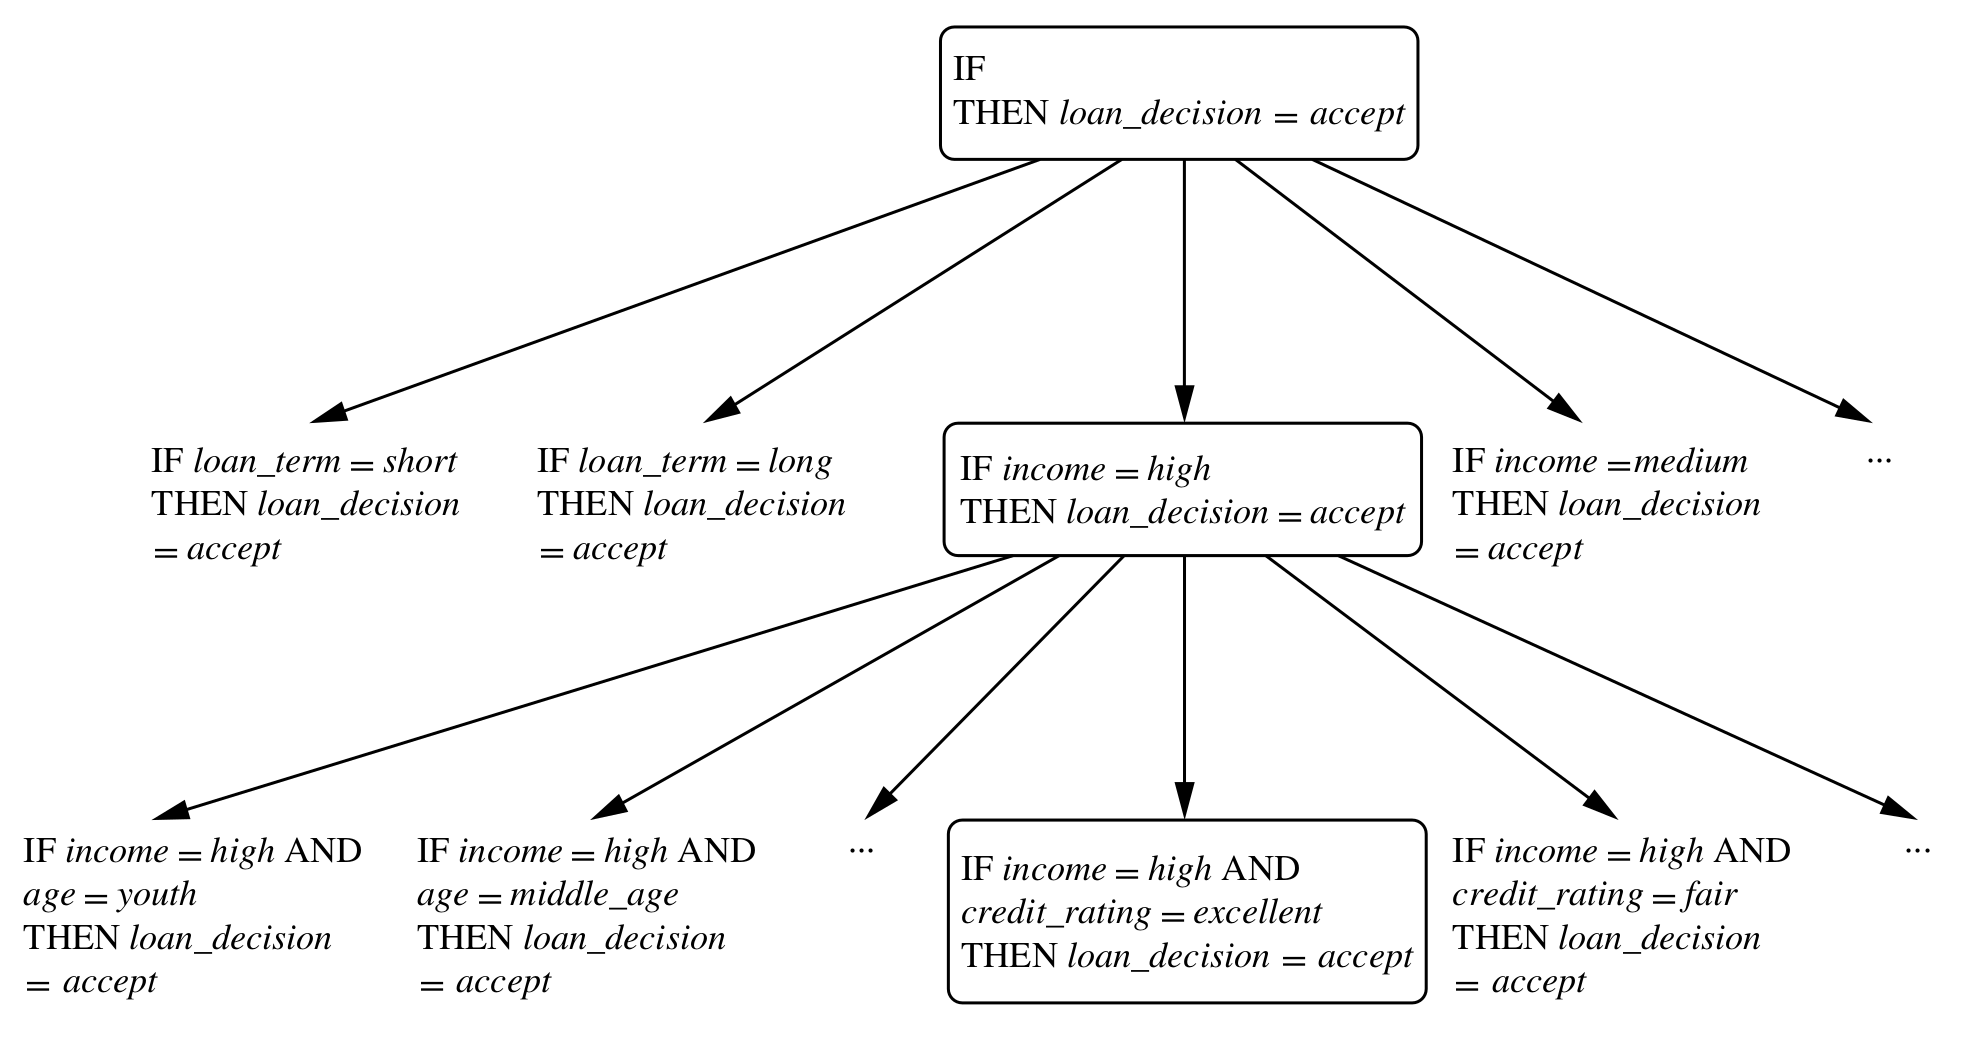
\includegraphics[height=0.8\textheight]{img/7-classification_rule_space.png}
	\end{figure}
\end{frame}

\begin{frame}{Sequential Covering Algorithm (IV)}
	\begin{itemize}
		\item \texttt{learn\_one\_rule} requires a measure of rule quality.
		\item Accuracy and coverage seems obvious choices on their own, but
		      individually not enough.
		\item \textbf{FOIL} (First-Order Inductive Learner): based on information gain
		      \begin{itemize}
			      \item Suppose we have two rules:
			            \begin{align*}
				            \label{}
				            R  & : \text{IF condition THEN class} = c  \\
				            R' & : \text{IF condition' THEN class} = c
			            \end{align*}
			      \item $pos/neg$ are $\#$ of positive/negative tuples covered by $R$, $pos'/neg'$ respectively for $R'$.
			      \item FOIL assesses the information gained by extending \textit{condition'} as
			            \begin{align*}
				            \text{FOIL\_Gain} = \text{pos}' \left( \log_2 \frac{\text{pos}'}{\text{pos}' + \text{neg}'} - \log_2 \frac{\text{pos}}{\text{pos}+\text{neg}} \right).
			            \end{align*}
			      \item FOIL favors rules that have high accuracy and cover many positive tuples.
		      \end{itemize}
	\end{itemize}
\end{frame}

\begin{frame}{Rule Pruning}
	\begin{itemize}
		\item \textbf{Danger of {\color{airforceblue}overfitting}.}
		\item \textbf{Removing a conjunct (attribute test),}
		      \begin{itemize}
			      \item if pruned version of rule has greater quality,\\
			            assessed on an independent set of test tuples (called "pruning set").
		      \end{itemize}
		\item \textbf{FOIL uses:}
		      \begin{align*}
			      \text{FOIL\_Prune}(R) = \frac{\text{pos}-\text{neg}}{\text{pos}+\text{neg}}.
		      \end{align*}
		\item If $\text{FOIL\_Prune}$ is higher for the pruned version of $R$, prune $R$.
	\end{itemize}
\end{frame}
